\documentclass{article}
\usepackage[utf8]{inputenc}
\usepackage[greek,english]{babel}
\usepackage{alphabeta}
\usepackage{fancyhdr}
\usepackage{listings}
\usepackage{mathtools}
\usepackage{xcolor}
\usepackage{biblatex}
\usepackage[left=2cm,right=2cm]{geometry}

\lstset {
        basicstyle=\ttfamily,
        columns=fullflexible,
        breaklines=true,
        keepspaces=true
}

\title{Σχεδίαση Ψηφιακών Συστημάτων - Εργασία Θεωρίας (Μέρος 1)}
\author{Χρήστος Μαργιώλης}
\date{Ιούλιος 2020}

\begin{document}

\begin{titlepage}
        \maketitle
\end{titlepage}

\renewcommand{\contentsname}{Περιεχόμενα}
\tableofcontents

\section{Κώδικας και τεκμηρίωση}

\subsection{\lstinline{mux2to1.vhd}}

Το παρακάτω κύκλωμα υλοποιεί έναν πολυπλέκτη 2-σε-1. Η υλοποίηση της
αρχιτεκτονικής του έχει ως εξής: αν η είσοδος \lstinline{s} έχει
τιμή 1, τότε θέτουμε στην έξοδο \lstinline{d} την τιμή της εισόδου
\lstinline{a}, ειδάλλως της \lstinline{b}. \\

\lstinputlisting[language=VHDL]{../mux2to1.vhd}
\pagebreak

\subsection{\lstinline{dec2to4.vhd}}

Το παρακάτω κύκλωμα υλοποιεί έναν αποκωδικοποιητή 2-σε-4 -- δηλαδή έχουμε
είσοδο 2 bit και δημιουργούμε μία έξοδο 4 bit. Για την υλοποίηση του 
χρησιμοποιούμε τις λογικές εξισώσεις του αποκωδικοποιητή:
\[D_0 = \overline{A_0 A_1}\]
\[D_1 = \overline{A_0} A_1\]
\[D_2 = A_0 \overline{A_1}\]
\[D_3 = A_0 A_1\] \\

\lstinputlisting[language=VHDL]{../dec2to4.vhd}
\pagebreak

\subsection{\lstinline{mux2to1gen.vhd}}

Στο παρακάτω κύκλωμα ξαναϋλοποιούμε τον πολυπλέκτη 2-σε-1, απλώς αυτή
την φορά παραμετροποιούμε τις εισόδους και εξόδους του ώστε να τον
μετατρέψουμε σε πολλαπλό πολυπλέκτη. Στην προκειμένη περίπτωση η παράμετρος
\lstinline{sz} έχει την τιμή 4, οπότε έχουμε έναν τετραπλό πολυπλέκτη
2-σε-1. \\

\lstinputlisting[language=VHDL]{../mux2to1gen.vhd}
\pagebreak

\subsection{\lstinline{mux2to1gen_tb.vhd}}

Στο παρακάτω κύκλωμα δοκιμάζουμε την λειτουργία του προηγούμενου κυκλώματος
με τη χρήση testbench. Η δημιουργία ενός testbench έχει ως εξής:
\begin{itemize}
	\item Ορίζουμε ένα άδειο entity για το testbench.
	\item Στην αρχικτεκτονική ορίζουμε την περιγραφή του κυκλώματος
		που θέλουμε να δοκιμάσουμε ως component, στην προκειμένη 
		περίπτωση τον πολλαπλό πολυπλέκτη 2-σε-1.
	\item Δημιουργούμε σήματα ίδιου τύπου για κάθε ένα από τα στοιχεία του
		component.
	\item Αντιστοιχούμε τα σήματα με τα πεδία του κυκλώματος (port map).
	\item Δημιουργούμε process και δίνουμε τιμές στα σήματα.
\end{itemize}

\lstinputlisting[language=VHDL]{../mux2to1gen_tb.vhd}
\pagebreak

\section{Εκτέλεση}

Οι παρακάτω κυματομορφές αφορούνε το testbench για τον πολλαπλό πολυπλέκτη 2-σε-1: \\

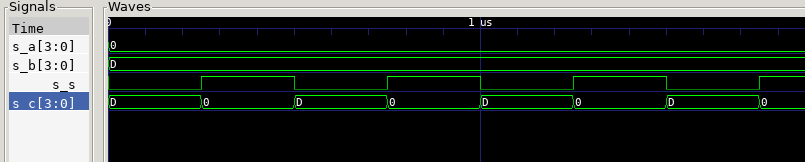
\includegraphics[width=\textwidth]{res/mux2to1gen.png}

\end{document}
